\documentclass{article}
\usepackage{tikz}
\usepackage{amsmath}
\usetikzlibrary{decorations.pathmorphing} % For coil spring

\begin{document}

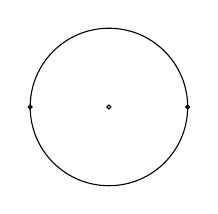
\begin{tikzpicture}

% Draw a simple circle
\draw (0,0) circle (1cm);
\node[circle,draw=black,fill=none,inner sep=0.5pt] at (0,0) {};
\node[circle,draw=black,fill=none,inner sep=0.5pt] at (-1,0) {};
\node[circle,draw=black,fill=none,inner sep=0.5pt] at (1,0) {};


% Coordinate points
\coordinate (O) at (0,0);
% \coordinate (M1) at (0,1.5);
% \coordinate (M2) at (0,0);
% \coordinate (A) at (-2,1.5);
% \coordinate (B) at (2,1.5);
% \coordinate (C) at (0,1.5);
% \coordinate (P) at (0,2.25);

\end{tikzpicture}

\end{document}